\section{Opportunities and Analysing a Architecture for Video Streaming Provisioning}
\label{sec:system-archi}

%{\color{blue} This section explains the architecture system, and what it is  for, explaining some protocols flowcharts. Studying the protocols and focusing in the system part of the experiments.}

%This section explains the modeling used in our experiments. We first provide an overview of the proposed video streaming service impacts in multi-tier networks. The remaining subsections describe the implementation of this service architecture.
In this section, as a preliminary result obtained with a multi-tier network experiment,  the QoE impact over a video streaming service is assessed. Thereafter, we describe some facts about the QoE characteristics and insights on the opportunities of caching multimedia content in edge nodes in terms of multi-tier networks. Designing a vertically edge cache hierarchies with N levels has Improve the QoE of users, serving the requested content as close to the user as possible; \textit{ii)} Reduce congestion at the core of the network, since it represents an operational overhead for the content provider; \textit{iii)} Efficiently forwarding requests between parent edge nodes whithin the hierarchy, to balance the video traffic in terms of hop counts and users attended. 


\subsection{Impact of Fog Multi-tier Network Approach}

To confirm these diference in users performance requesting a video from a node in different tiers, we present two users requesting a multimedia content in different layers. Then an analyses of the impacts over the network is addressed. In Figure~\ref{fig:impact-two-layers}, the graphs show the results of bitrate, interruptions, buffer and representations switch, respectively from left to the right.%and along x-axis the simulation time. 
The Figure illustrate a two tier network model. When a client requests the video of a cache edge node, it can located in layer L1 or L2. Where each layer level has different network factors, e.g., load, latency, etc. For instance, a L1 layer can be a personal computers, laptops and smartphones, where the node retransmits the video content by means of wired or wireless communication. Whereas in L2 layer
a specific Edge gateways can be distributed on local fog nodes, for example.

\begin{figure}
    \centering
    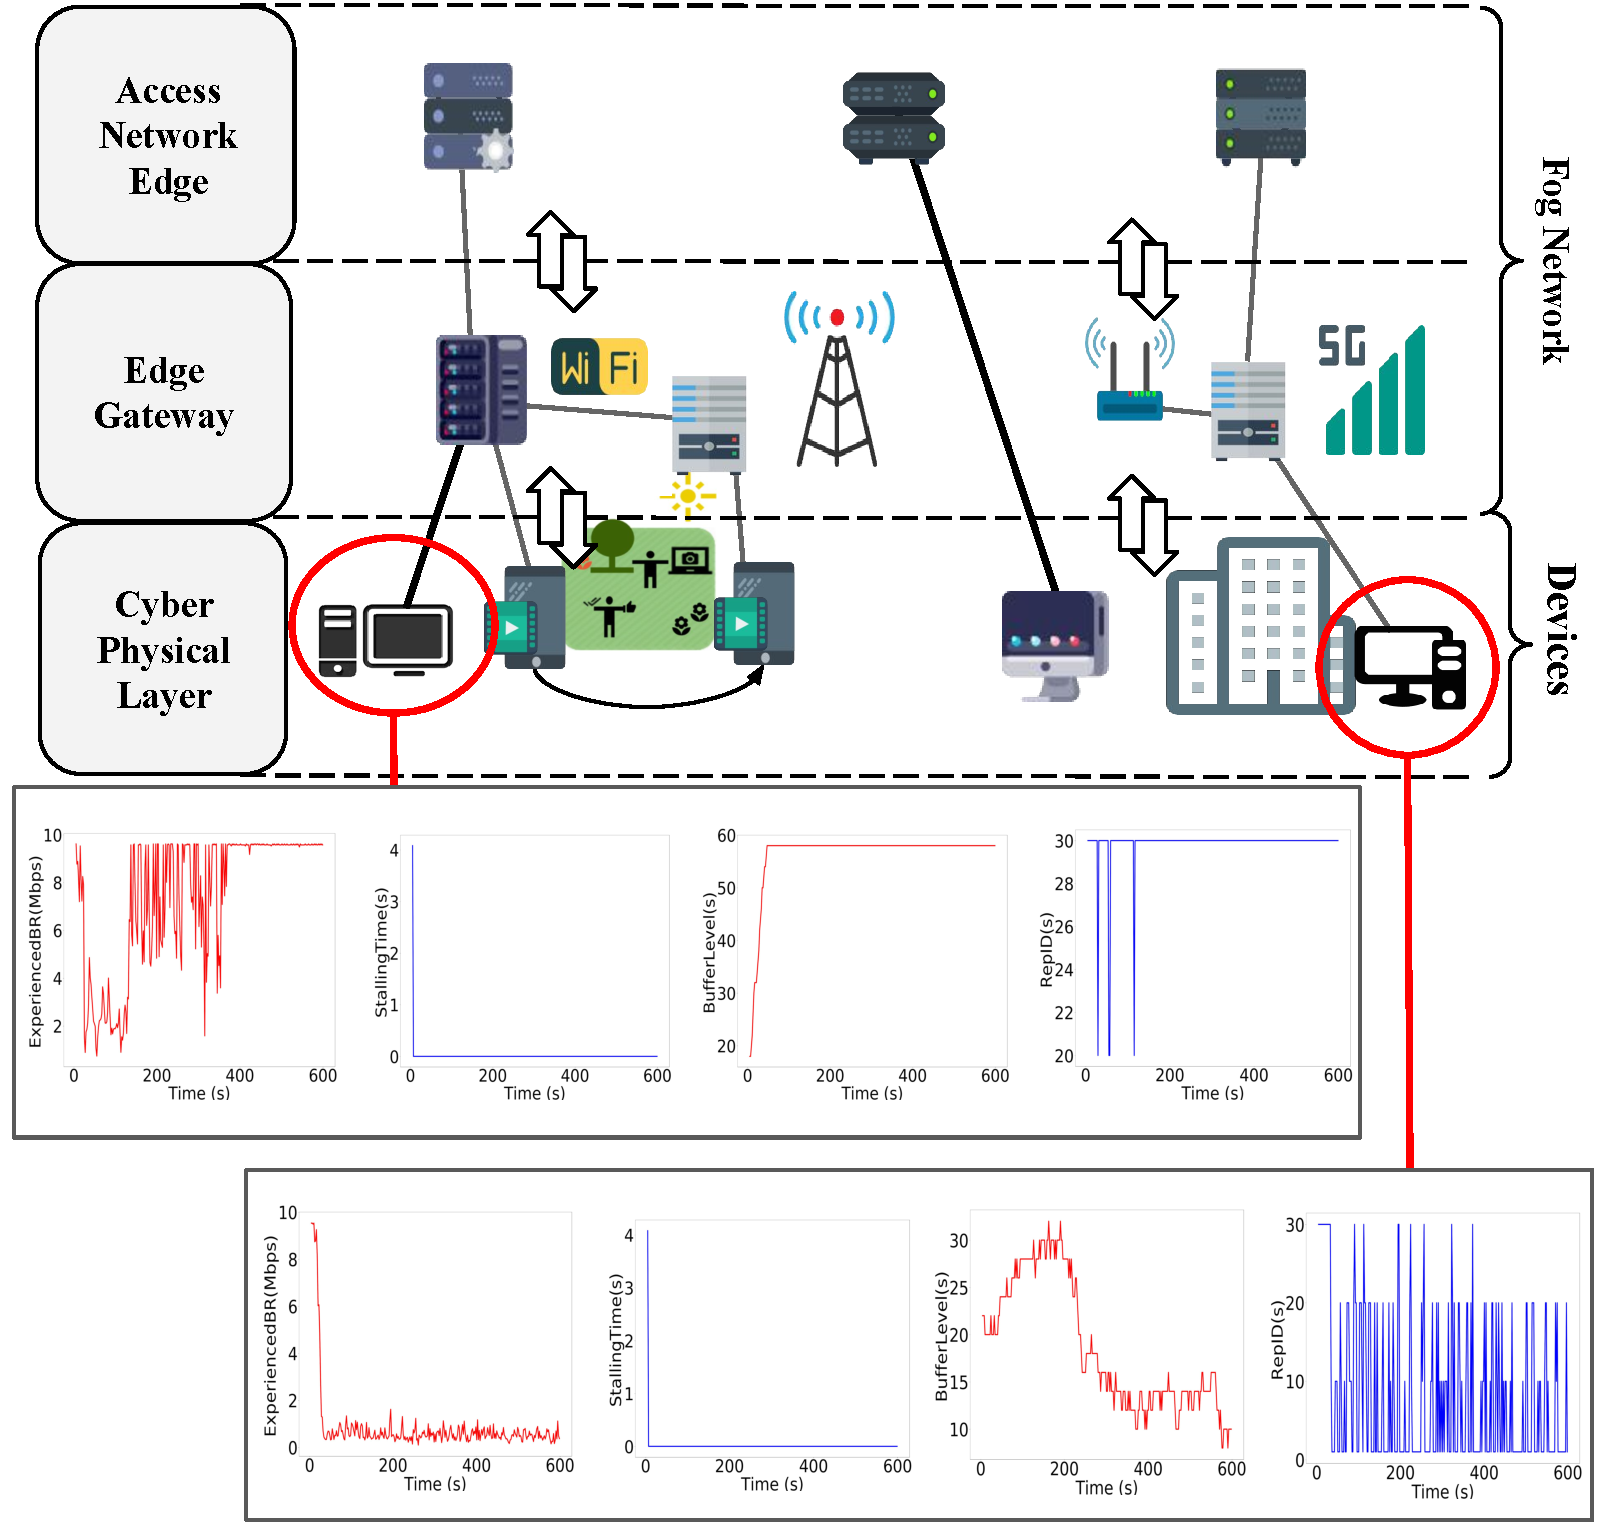
\includegraphics[width=0.9\linewidth]{images/qoe-multi-level.pdf}
    \caption{\textbf{The number of bitrate switches, stalls, buffer size, the startup delay in seconds of a DASH player requesting a video with 10 bitrate levels varying from 50 to 4,500Kbps and from nodes in different tiers.}}
    \label{fig:impact-two-layers}
\end{figure}


As we can see, both users have had no interruptions throughout the video, besides the initial interruption until the start of the video. However, the user who received the video on the nearest fog layer had a higher bit rate than the other user. As well as the buffer was soon filled and the user had the best possible resolution of the video. Whereas the user who received the video from a more distant layer, in some moments, worked with the buffer at the limit and had to constantly switch resolutions so that there is no interruption during the video execution. Both users received a same from different Layers, even without any interruptions during the video transmission, a video comes from differnet layers impacts directly the users' QoE.


\subsection{Multi-tier Edge-Cloud Network Opportunities}

%Esta seção apresenta algumas oportunidades dentro de redes multi-tier edge/cloud para o provisionamento da transmissção de videos. Aproveitar nós próximos aos usuários podem melhorar o funcionamento do rede como um todo, aqui nós discutimos alguns insights que podem ser usados em favor dos stakeholders que utilizam a infraestrutura para transmissão de video. 
This section presents some opportunities within multi-tier edge/cloud networks for the provision of video transmission. Taking advantage of nodes close to users can improve the functioning of the network as a whole, here we discuss some insights that can be used in favor of stakeholders who use the infrastructure for video transmission


\subsubsection{Improving User QoE}

%the cloud distributes the video content to the different levels of the edge. Depending the level which the video is cached the users' experience changes. The architecture is based on held the video distribution with QoE support. The work divides the edge into three layers, to guarantee coverage, storage, upload and download capacity. 
Inside a multilevel environment composed of more than one domain of devices, the domain resources can be used to host the video content in close proximity to the end users, reducing latency and mitigating the load on the main cloud networks. To integrate video streaming services in such communication environments, the fog nodes are composed of specific resources that can be combined to carry out the video transmission. Within this context, mechanisms for integrating schemes and video streaming rises an opportunitie to improve QoE.% at each level of the network.
The results reported in Fig~\ref{fig:impact-two-layers} shows that is possible improve the users staisfaction using the edge multi-tier network. Dependendo do nível de alocação do serviço de video, a variação na suavização do video entre caracteristicas do reprodutor muda. 

\subsubsection{Potential Bandwith Saving}
%Video Caching, Analytics, and Delivery at the Wireless Edge: A Survey and Future Directions
Videos streamed in higher quality increase network bandwidth, consequently, a provisioning from the Cloud will incur high communication expenses. 
The process of delivery part of the video along the network can significantly save bandwidth utilization. Instead of sending all frames to the edge server or by lowering the encoding quality of uninteresting portions of the frames. Different delivery approaches can have different performances to reduce the uplink bandwidth. Moreover, none of the surveyed articles have considered the end-to-end design of live streaming, wherein the edge server adapts the video streams based on both uplink and downlink bandwidth capacities. Additionally, new forms of video content are being generated today.


\subsubsection{Cacheability}

Caching audio/video during peak hours ...
Manage the QoE users refer to those service where the satisfaction guarantees can be centrally controlled by the controller. The Controller can address this problem by creating a control channel to managed-quality video streaming services over the edge-cloud network.